\documentclass[final]{beamer}

\usetheme{enziteto}

\usepackage[orientation=portrait, size=a0, scale=1.4, debug]{beamerposter}
\usepackage{booktabs}
\usepackage{dcolumn}
\usepackage{colortbl}
\usepackage{xcolor}
\usepackage{hyperref}
\usepackage{amsmath}
%\usepackage[absolute, showboxes, overlay]{textpos}
\usepackage[absolute, overlay]{textpos}
\usepackage{calc}
%\usepackage[colorgrid,texcoord]{eso-pic}
\usepackage{biblatex}
% \usepackage{enumitem}
\defaultfontfeatures{Mapping=tex-text}

\addbibresource{../referomnia/referomnia.bib}

\usepackage{blindtext}


\newcommand*\mccol[2]{\multicolumn{#1}{c}{#2}}
\newcommand*\tmccol[2]{\mccol{#1}{\tiny\textsf{#2}}}
\newcommand*\bmccol[2]{\mccol{#1}{\textbf{#2}}}


% \usepackage{xparse}
% \ExplSyntaxOn
% \NewDocumentCommand{\convertto}{mm}
% % #1 = em or ex (or any other unit)
% % #2 = dimen to convert
% {
%   \texttt{#2~=~\fp_to_decimal:n { round ( #2/1#1, 5 ) }#1}
% }
% \DeclareExpandableDocumentCommand{\thelength}{ O{mm} m }
% {
%   \fp_to_decimal:n { round ( #2/1#1, 5 ) } #1
% }
% \ExplSyntaxOff


% 
% custom colors
\definecolor{untractable_red}{RGB}{209, 25, 25}
\definecolor{tractable_green}{RGB}{0, 153, 51}


\setbeamertemplate{itemize item}{\raisebox{.21ex}{\hbox{\tiny\textcolor{lacamlilac}{$\boldsymbol{\oplus}$}}\hspace{0pt}}}
\setbeamertemplate{itemize subitem}{\raise .2ex\hbox{\tiny\textcolor{lacamlilac}{$\boldsymbol{\otimes}$}}\hspace{0pt}}
\setbeamertemplate{itemize subsubitem}{\textcolor{lacamlilac}{$\oplus$}}
\setbeamertemplate{bibliography item}{\hspace{10pt}\raise .2ex\hbox{\tiny\textcolor{lacamlilac}{$\boldsymbol{\oplus}$}}}


% \setbeamertemplate{headline}{}

% \addbibresource{../referomnia/referomnia.bib}

\title{Simplifying, Regularizing and Strengthening Sum-Product Network Structure Learning}
\author{Antonio  Vergari, Nicola  {Di Mauro} and Floriana Esposito}
\date{}


\begin{document}

\institute{Università degli Studi di Bari}
\department{Dipartimento di Informatica}
\laboratory{LACAM}
\group{Machine Learning}
\institutelogo{
\includegraphics[width=25pt]{figures/unibaba}}
\lablogo{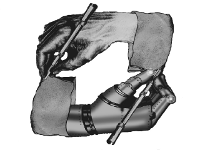
\includegraphics[width=35pt]{figures/lacam}}


% {
%   \setbeamertemplate{headline}{}
%   \setbeamertemplate{footline}{}
%   \begin{textblock}
%     \titlepage
%   \end{textblock}
% }

\newcommand{\hmargin}{20mm}
\newcommand{\vmargin}{20mm}
\textblockorigin{\hmargin}{\vmargin}

\setlength{\TPHorizModule}{1cm}
\setlength{\TPVertModule}{1cm}

%
% TODO: generalize this
\newlength{\posterwidth}
\setlength{\posterwidth}{841mm - 2\hmargin}
\newlength{\posterheight}
\setlength{\posterheight}{1189mm}

\newcommand{\ncols}{3}
\newlength{\colwidth}
\setlength{\colwidth}{\posterwidth/\ncols}


\newlength{\colhpoint}


\begin{frame}{}
  %
  % title
  % \textblockcolour{header}
  \begin{textblock}{58}(0, 0)
    \usebeamerfont{section name}
    \huge
    Simplifying, Regularizing and Strengthening\\
    Sum-Product Network Structure Learning
  \end{textblock}
  %
  % authors
  \begin{textblock}{30}(0, 6.5)
    \usebeamerfont{author}
    \small
    Antonio  Vergari, Nicola  {Di Mauro} and Floriana Esposito
  \end{textblock}
  % 
  % email
  \begin{textblock}{15}(30, 6.5)
    \usebeamerfont{author}
    \small
    \emph{\{firstname.lastname@uniba.it\}}
  \end{textblock}
  %
  % affiliations
  \begin{textblock}{20}(60, 0)
    \usebeamerfont{author}
    \scriptsize
    \begin{minipage}[t]{5cm}
      \vspace{0pt}\hspace{10pt}
      
\includegraphics[width=90pt]{figures/unibaba}
    \end{minipage}
    \begin{minipage}[t]{12cm}
    \vspace{27pt}
      \flushleft
      University of Bari "Aldo Moro", Italy\\
    \vspace{2pt}
      Department of Computer Science
    \end{minipage}\\[0.75cm]
    \usebeamerfont{author}
    \scriptsize
    \begin{minipage}[t]{5cm}
      \vspace{0pt}
      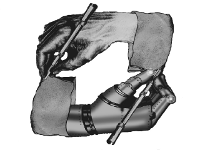
\includegraphics[width=110pt]{figures/lacam}
    \end{minipage}
    \begin{minipage}[t]{12cm}
      \vspace{23pt}
      \flushleft
      LACAM\\
      \vspace{2pt}
      Machine Learning
    \end{minipage}
  \end{textblock}
  
  
  %
  % section 1
  \begin{textblock}{80}(0, 10.5)
    \usebeamerfont{section name}
    Sum-Product Networks and Tractable Models
  \end{textblock}
  
  
  \begin{textblock}{25.2}(0, 13)
    \footnotesize
    Probabilistic Graphical Models (PGMs) provide a tool to compactly
    represent joint probability distributions $P(\mathbf{X})$.

    However, \emph{\textbf{inference}}, the main task one may want to perform on a PGM, is generally \emph{\textbf{untractable}}.\bigskip  
    \begin{table}[!ht]
      \setlength{\tabcolsep}{10pt}
      \centering
      \begin{tabular}{c c c c}
        \scriptsize\color{untractable_red}  \textbf{\emph{untractable}} & \scriptsize\color{untractable_red} \textbf{\emph{untractable}}& \scriptsize\color{tractable_green} \emph{\textbf{tractable}} & \scriptsize\color{tractable_green} \emph{\textbf{tractable}}\\

        
        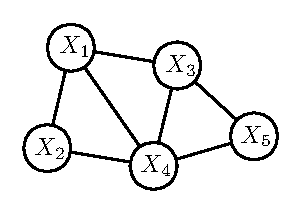
\includegraphics[width=0.22\linewidth]{figures/mrf} &
        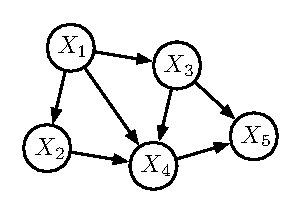
\includegraphics[width=0.22\linewidth]{figures/bn} &
        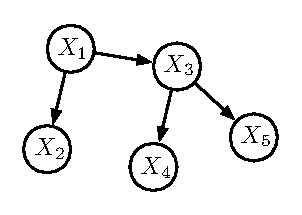
\includegraphics[width=0.22\linewidth]{figures/clt} &
        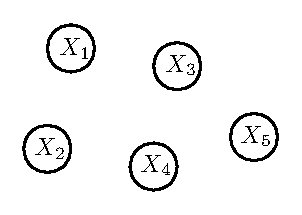
\includegraphics[width=0.22\linewidth]{figures/nf}\\                                                             
        \addlinespace[-0.2cm]
        % \scriptsize  $P(\mathbf{X})=\frac{1}{Z}\prod_{c}\phi_{c}(\mathbf{X}_{c})$ & 
        % \scriptsize  $P(\mathbf{X})=\prod_{i=1}^nP(X_{i}|\mathbf{Pa}_{i})$&
        %                                                                  %           \addlinespace[0.5cm]
                                                                            
        %                                                                     %\addlinespace[-0.2cm]
        % \scriptsize $P(\mathbf{X})=\prod_{i=1}^nP(X_{i}|Pa_{i})$ &
        % \scriptsize $P(\mathbf{X})=\prod_{i=1}^nP(X_{i})$ \\                                                             
        \tiny  $P(\mathbf{X})=\frac{1}{Z}\prod\limits_{c}\phi_{c}(\mathbf{X}_{c})$ & 
        \tiny  $P(\mathbf{X})=\prod\limits_{i=1}^nP(X_{i}|\mathbf{Pa}_{i})$&
        % \addlinespace[0.5cm]
        \tiny $P(\mathbf{X})=\prod\limits_{i=1}^nP(X_{i}|Pa_{i})$ &
        \tiny $P(\mathbf{X})=\prod\limits_{i=1}^nP(X_{i})$                                                              
      \end{tabular}\bigskip
      
    \end{table}

    To ensure polynomial inference, tractable models trade off
     expressiveness.
  \end{textblock}
  
  \begin{textblock}{25.2}(27.4, 13)
    \footnotesize
    Sum-Product Networks (SPNs) are DAGs
    \emph{compiling} a pdf $P(\mathbf{X})$ into a \textbf{\emph{deep}} architecture of \textbf{sum}
    and \textbf{product} nodes over univariate distributions $X_1,\dots,X_n$ as leaves.
    The parameters of the network are the weights $w_{ij}$ associated to sum
    nodes children edges.\par
    
    Product nodes define factorizations over independent vars, sum
    nodes mixtures.\par
    
    % Sum node children weights are the parameters of the model.\\
    
    Products over nodes with different scopes (\emph{decomposability}) and
    sums over nodes with same scopes (\emph{completeness}) guarantee modeling
    a pdf (\emph{validity}).\par\bigskip
    
    
    \begin{minipage}{0.5\linewidth}
      \centering
      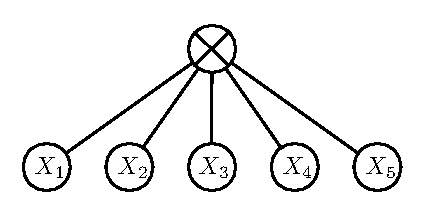
\includegraphics[width=0.65\linewidth]{figures/spn-prod}
    \end{minipage}\begin{minipage}{0.5\linewidth}
      \centering
      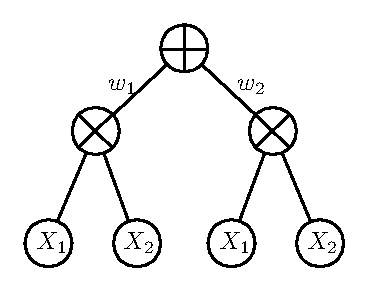
\includegraphics[width=0.55\linewidth]{figures/spn-sum}
    \end{minipage}
    
    
  \end{textblock}

  % \begin{textblock}{25}(34.1, 15.3)
  %   \small
  %     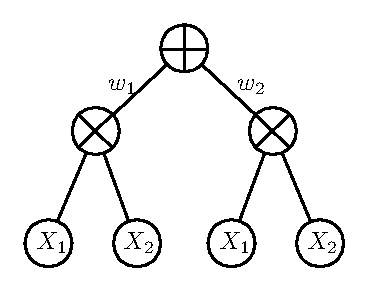
\includegraphics[width=0.7\linewidth]{figures/spn-sum}
  % \end{textblock}
  
  \begin{textblock}{25.2}(54.8, 13)
    \footnotesize
    \begin{minipage}{0.7\linewidth}
    
    Bottom-up evaluation of the network:
    $$S_{X_i}(x_j)=P(X_i=x_j)$$    
    $$S_{+}(\mathbf{x})=\sum\limits_{i\in
      ch(+)}w_{i}S_{i}(\mathbf{x})\quad S_{\times}(\mathbf{x})=\prod\limits_{i\in
      ch(\times)}S_{i}(\mathbf{x})$$\\[10pt]
    \setlength{\leftmargini}{30pt}
    Inferences linear in the \emph{\textbf{size of the network}} (\emph{\# edges}):
    \begin{itemize}
    \item $Z = S(*)$ (all leaves output 1)
    \item $P(\mathbf{e}) = S(\mathbf{e})/S(*)$
    \item $P(\mathbf{q}| \mathbf{e}) = \frac{P(\mathbf{q},
        \mathbf{e})}{P(\mathbf{e})} = \frac{S(\mathbf{q},
        \mathbf{e})}{S(\mathbf{e})}$
    \item $MPE(\mathbf{q},\mathbf{e}) = \max_{\mathbf{q}}P(\mathbf{q},
      \mathbf{e}) = S^{max}(\mathbf{e})$, turning sum nodes into max nodes
    \end{itemize}
  \end{minipage}\begin{minipage}{0.28\linewidth}
    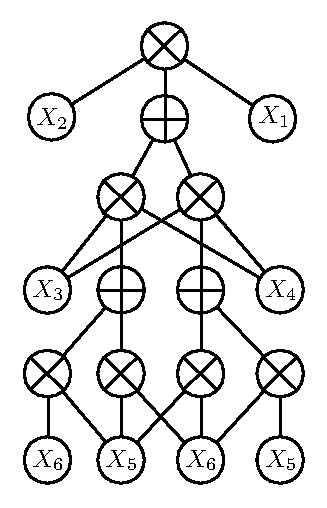
\includegraphics[width=0.8\linewidth]{figures/spn-long}
  \end{minipage}\\[20pt]

  The \emph{\textbf{depth of the network}} (\emph{\# layers})
  determines expressive efficiency~\parencite{Martens2014,Zhao2015}.

  \end{textblock}
  
  %
  % section 2
  \begin{textblock}{80}(0, 29.2)
    \usebeamerfont{section name}
    How and why to perform structure learning
    
  \end{textblock}
  
  \begin{textblock}{25.2}(0, 31.7)
    \footnotesize
     
    SPN structure learning is a constraint-based
    search. Main ideas: to discover hidden variables for sum nodes and independences
    for product nodes by applying some form of clustering
    along matrix axis. Different variations:
    using K-Means on
    features~\emph{\parencite{Dennis2012}}; merging features bottom-up
    with IB heuristics\emph{~\parencite{Peharz2013}};
    \emph{\textbf{LearnSPN}}~\emph{\parencite{Gens2013}} is the first principled top-down greedy
    algorithm. 
    

    % \begin{itemize}
    %   \itemsep 6pt
    % \item greedy top-down: KMeans on features~\emph{\parencite{Dennis2012}};
      
    % \item greedy bottom up: merging feature regions by a \emph{Bayesian-Dirichlet independence test},  and reducing edges by maximizing MI\emph{~\parencite{Peharz2013}}

    % \item \textbf{ID-SPN}: turning LearnSPN in log-likelihood guided expansion of sub-networks
    %   approximated by Arithmetic Circuits~\emph{\parencite{Rooshenas2014}}
      
    % \end{itemize}
  \end{textblock}
  
  \begin{textblock}{25.2}(27.4, 31.7)
    \footnotesize
    LearnSPN builds a tree-like SPN by recursively splitting the data
    matrix: columns in pairs by a greedy \textbf{\emph{G Test}} based
    procedure with threshold $\rho$: $G(X_i, X_j) =  2\sum_{x_i \sim
      X_i}\sum_{x_j \sim X_j}c(x_i, x_j)\cdot \log\frac{c(x_i,
      x_j)\cdot |T|}{c(x_i)c(x_j)}$ (Figure 1.c); instances in
    $|C|$ clusters with \textbf{\emph{online Hard-EM}} (Figure 1.b) with cluster number penalty
    $\lambda$: $Pr(\mathbf{X})= \sum_{C_i \in \mathbf{C}}\prod_{X_j
      \in \mathbf{X}}Pr(X_j,C_i)$. Weights are the cluster proportions.

    % \begin{itemize}
    % \item splitting columns in pairs by a greedy \textbf{\emph{G Test}} based
    %   procedure with threshold $\rho$:
    %   \[
    %   G(X_i, X_j) =  2\sum_{x_i \sim X_i}\sum_{x_j \sim X_j}c(x_i, x_j)\cdot \log\frac{c(x_i, x_j)\cdot |T|}{c(x_i)c(x_j)}
    %   \]
 
    %   \end{itemize}
  \end{textblock}
  
  
  \begin{textblock}{60}(0, 37.4)
    \small
    \begin{minipage}[t][][t]{5.103cm}
      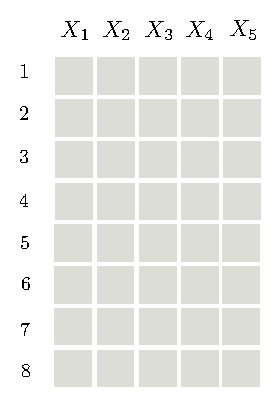
\includegraphics[width=\linewidth]{figures/grid-0}
    \end{minipage}\hspace{30pt}\begin{minipage}[t]{4.4874cm}
      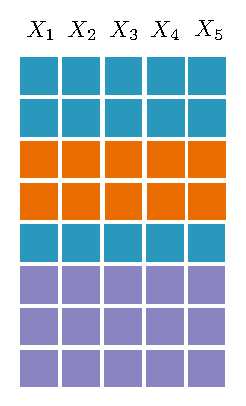
\includegraphics[width=\linewidth]{figures/grid-1}
    \end{minipage}\hspace{30pt}\raisebox{82pt}{\begin{minipage}[t]{5.67cm}\vspace{-120pt}
      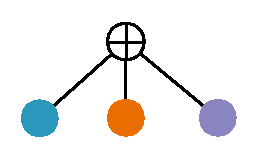
\includegraphics[width=\linewidth]{figures/learnspn-1}
    \end{minipage}}\hspace{30pt}\begin{minipage}[t]{4.4874cm}
      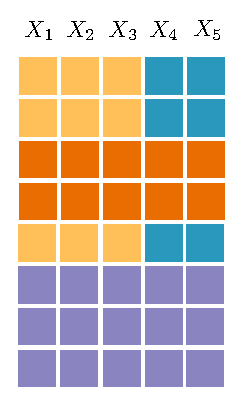
\includegraphics[width=\linewidth]{figures/grid-2}
    \end{minipage}\hspace{30pt}\raisebox{42pt}{\begin{minipage}[t]{6.48cm}
      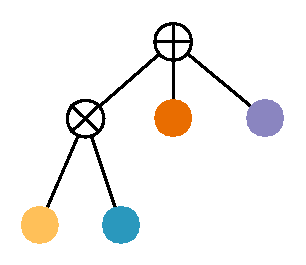
\includegraphics[width=\linewidth]{figures/learnspn-2}
    \end{minipage}}\hspace{30pt}\begin{minipage}[t]{4.6364cm}
    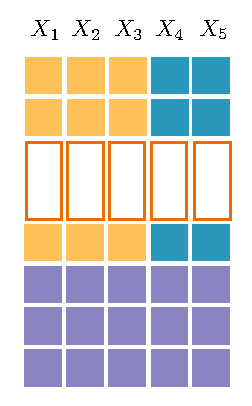
\includegraphics[width=\linewidth]{figures/grid-3}                                                               \end{minipage}\hspace{30pt}\raisebox{42pt}{\begin{minipage}[t]{8.1cm}
      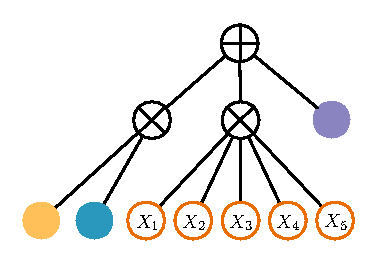
\includegraphics[width=\linewidth]{figures/learnspn-3}                                             
    \end{minipage}}\hspace{50pt}\raisebox{180pt}{\begin{minipage}[t]{4cm}
      \tiny\flushleft
      Figure 1.\\
      LearnSPN steps depiction starting from a full data matrix \emph{(a)},
      clustering on rows \emph{(b)}, then on columns \emph{(c)}, and putting a naive
      factorization on leaves \emph{(d)}
    \end{minipage}}\\
  \vspace{-20pt}\hspace{80pt}\begin{minipage}[t]{7cm}
    \scriptsize\emph{(a)}
  \end{minipage}\hspace{80pt}\begin{minipage}[t]{7cm}
    \scriptsize\emph{(b)}
  \end{minipage}\hspace{175pt}\begin{minipage}[t]{7cm}
    \scriptsize\emph{(c)}
  \end{minipage}\hspace{175pt}\begin{minipage}[t]{7cm}
    \scriptsize\emph{(d)}
  \end{minipage}
    
    % \begin{table}[ht]
    %   \centering
    %   \begin{tabular}{l l l l l l l}
    %     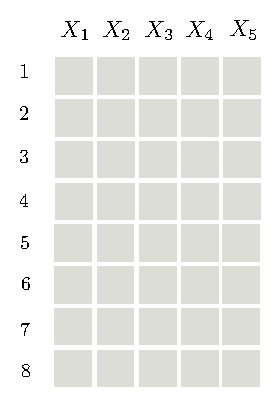
\includegraphics[width=0.228\linewidth]{figures/grid-0}&
    %     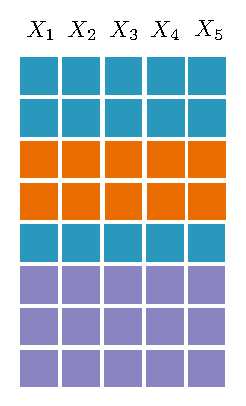
\includegraphics[width=0.2\linewidth]{figures/grid-1}&
    %     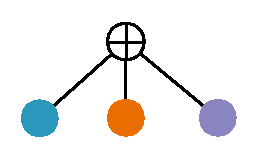
\includegraphics[width=0.2\linewidth]{figures/learnspn-1}&                                                       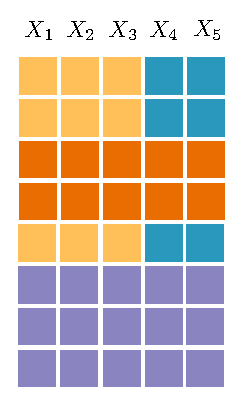
\includegraphics[width=0.2\linewidth]{figures/grid-2}&
    %     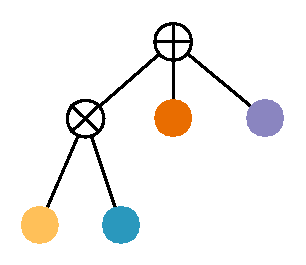
\includegraphics[width=0.24\linewidth]{figures/learnspn-2}&
    %     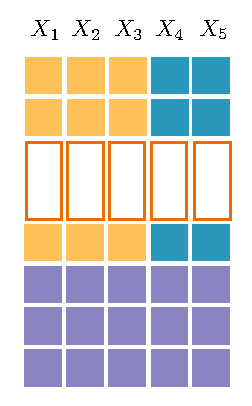
\includegraphics[width=0.208\linewidth]{figures/grid-3}&                                                          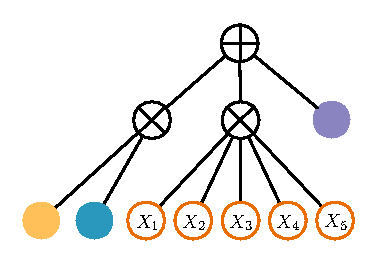
\includegraphics[width=0.30\linewidth]{figures/learnspn-3}\\                                             
    %   \end{tabular}
    % \end{table}
    
  \end{textblock}
  
  
  \begin{textblock}{25.2}(54.8, 31.7)
    \footnotesize
    If there are less than $m$ instances, it puts a \textbf{\emph{naive
        factorization}} over leaves (Figure 1.d). For each univariate distribution
    it gets its \emph{\textbf{ML estimation}} smoothed by $\alpha$. LearnSPN
    hyperparameter space is thus: $\{\rho, \lambda, m, \alpha\}$.\par\bigskip

   %  \small
  %   \begin{itemize}
  % \item clustering instances with \textbf{\emph{online Hard-EM}} with cluster penalty
  %   $\lambda$:
  %   \[\begin{array}{cc}
  %       Pr(\mathbf{X})= \sum_{C_i \in \mathbf{C}}\prod_{X_j \in \mathbf{X}}Pr(X_j|C_i)Pr(C_i)\\
  %       % & Pr(C_i) \propto e^{-\lambda |\mathbf{C}|\cdot |\mathbf{X}|}\\
  %     \end{array}\]
  %     weights are the proportions of instances falling into each cluster
  %   \item if there are less than $m$ instances, put a \textbf{\emph{naive
  %         factorization}} over leaves
  %   \item each univariate distribution get \emph{\textbf{ML
  %         estimation}} smoothed by $\alpha$  
  %   \end{itemize}

    The state-of-the-art, in terms of test likelihood, is \textbf{ID-SPN}: it turns LearnSPN in log-likelihood guided expansion of sub-networks
    approximated by Arithmetic
    Circuits~\emph{\parencite{Rooshenas2014-short}}. However it is
    overparametrized, and slower.\par\bigskip
    
    
    Tractability is guaranteed if the network size is polynomial in \#
    vars. \emph{\textbf{Structure quality matters}} as much as likelihood. comparing network sizes is more solid than comparing inference times.\par\bigskip

    LearnSPN is too greedy and the resulting SPNs are overcomplex
    networks that may not generalize well. \textbf{\emph{Structure quality desiderata}}: \emph{smaller} but \emph{accurate}, \emph{deeper} but not wider, SPNs. 

  \end{textblock}
  
  
  %
  % section 3
  \begin{textblock}{80}(0, 47.9)
    \usebeamerfont{section name}
    Simplifying by limiting node splits
  \end{textblock}

  % 
  % section 3.1
  \begin{textblock}{20}(54.8, 47.9)
    \usebeamerfont{section name}
    Experiments
  \end{textblock}
  
  \begin{textblock}{25.2}(0, 50.4)
    \footnotesize
    \setlength{\leftmargini}{30pt}
    \textsf{LearSPN} performs two interleaved \textbf{\emph{greedy
        hierarchical}} divisive \textbf{\emph{clustering}}
    processes. Each process benefits from the other one improvements
    and similarly suffers
    from the other's mistakes.\par\bigskip

    Idea: slowing down the processes by limiting the number of
    nodes to split into. \textsf{SPN-B}, variant of \textsf{LearnSPN} that uses EM
    for mixture modeling but doing only \textsf{B}inary splits for sum nodes children
    ($k=2$) when clustering rows.\par\bigskip
    
    \raisebox{55pt}{\begin{minipage}[t]{0.6\linewidth}
        \flushleft
    %  Objectives:
    %   \begin{itemize}
    %   \item not committing to complex structures too early  
    %   \item same expressive power: successive row splits can represent
    %     sum nodes with more than two children
    %   \item reducing node out fan increases the network depth 
    %   %\item same accuracy, smaller networks
    %   \end{itemize}
    % \end{minipage}}\hfill\begin{minipage}[c]{0.35\linewidth}
    %   \begin{center}
    %     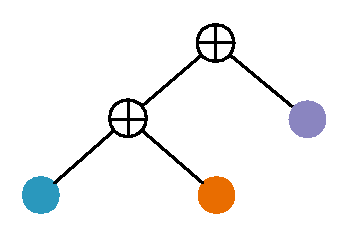
\includegraphics[width=0.85\linewidth]{figures/learnspn-4}
    %   \end{center}
    % \end{minipage}
    Objectives: not committing to complex structures too early while
    retaining same expressive power (right Figure is equivalent to the
    SPN in Figure 1.b); moreover, reducing
          the node out fan increases the network depth. Plus, there is no
          need for $\lambda$ anymore.
      \end{minipage}}\hspace{40pt}\begin{minipage}[c]{0.3\linewidth}
      \begin{center}
        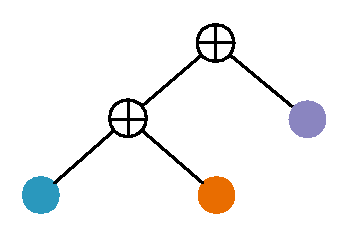
\includegraphics[width=7.5cm]{figures/learnspn-4}
      \end{center}
    \end{minipage}
      \end{textblock}
  
  \begin{textblock}{25.2}(27.4, 50.4)

    \footnotesize
    By increasingly limiting the max number of allowed splits the depth of the
    structures increases and the network size rate of growth
    decreases.  
    \begin{table}[ht]
      \setlength{\tabcolsep}{30pt}  
      \centering
      \begin{tabular}{c c}
        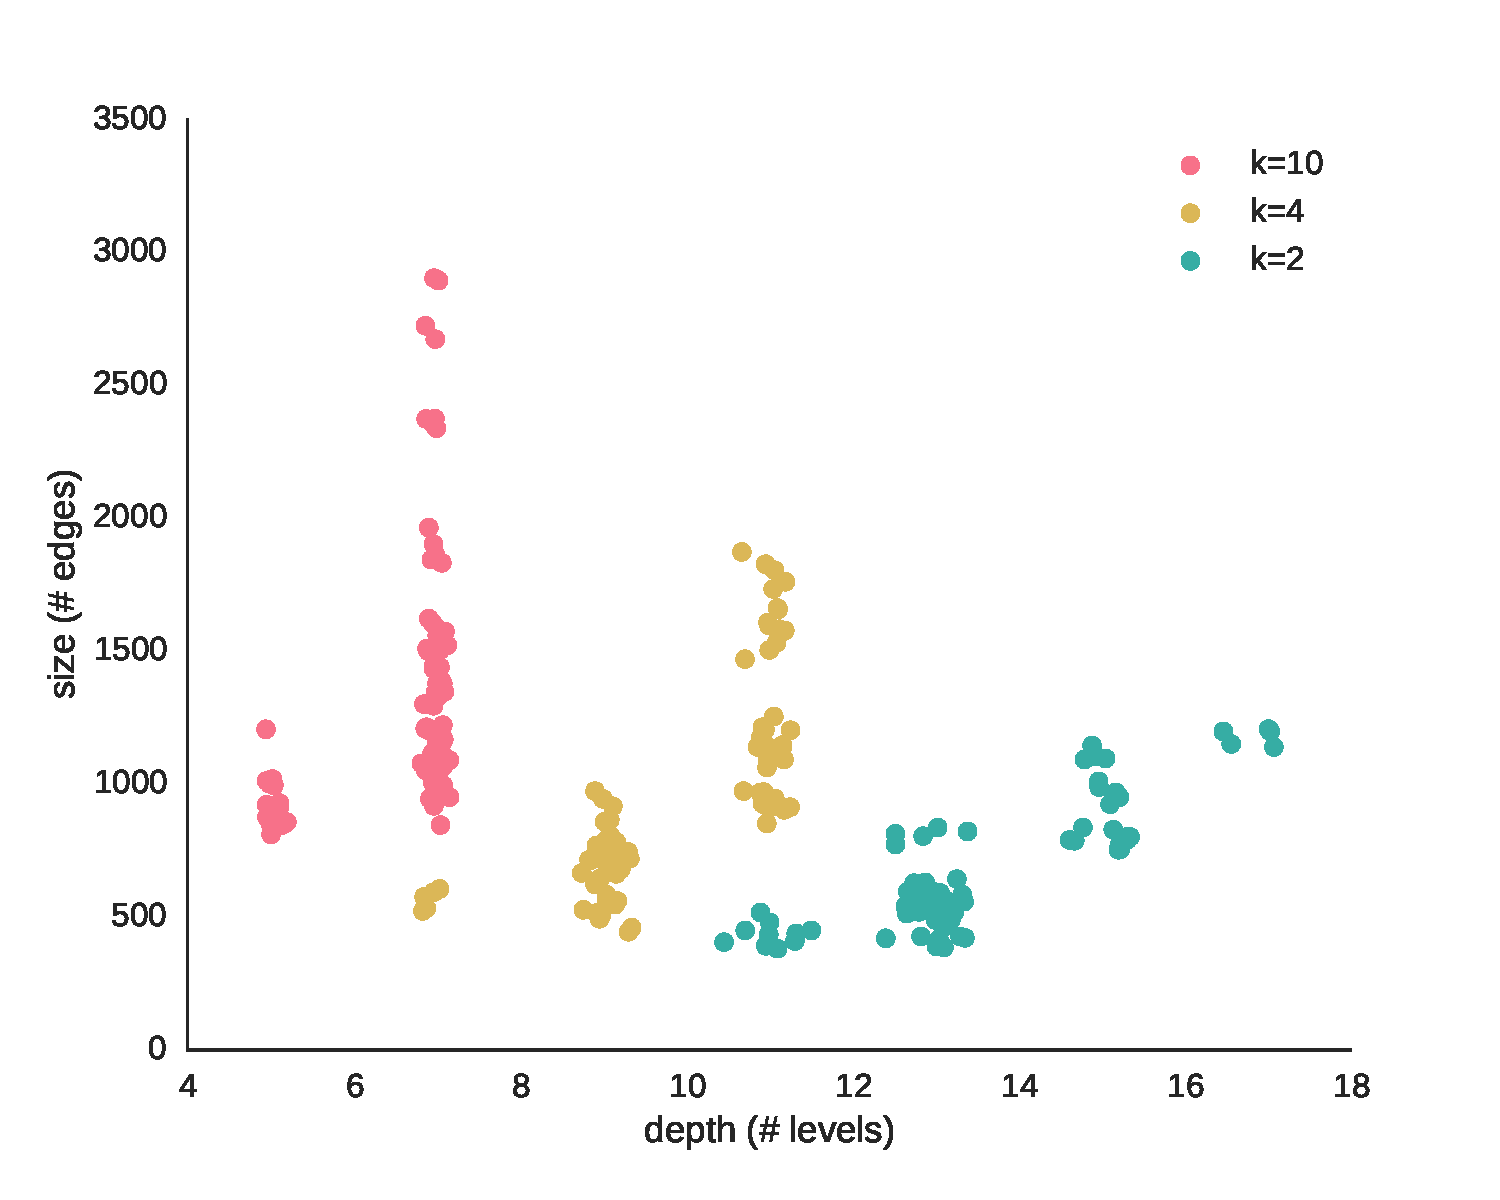
\includegraphics[width=0.4\linewidth]{figures/nltcs-depth.pdf}&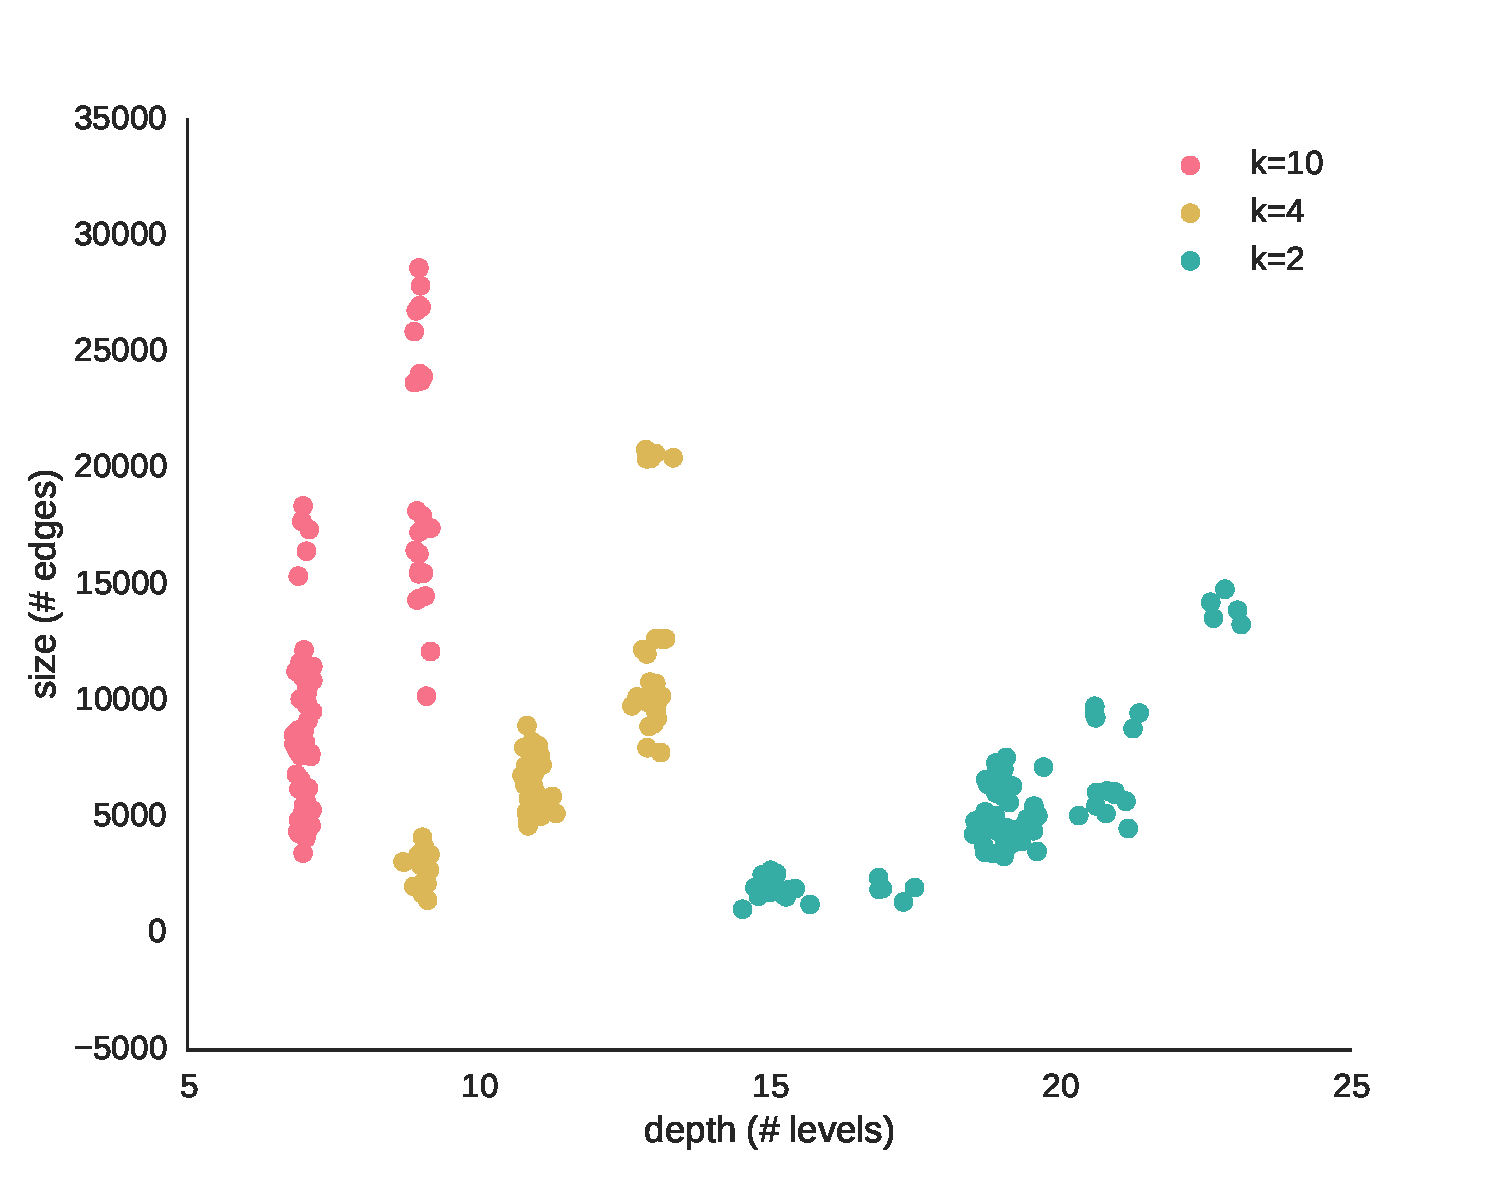
\includegraphics[width=0.4\linewidth]{figures/plants-depth.pdf}
      \end{tabular}
    \end{table}
    \vspace{-20pt}
    \begin{center}
      \begin{minipage}[t]{0.9\linewidth}
        \tiny\flushleft
        Figure 2. Comparing network sizes and depths while varying the max
        number of sum node children splits ($k\in\{10, 4, 2\}$). Each dot is an experiment
        in the grid search hyperparameter space performed by
        \textsf{SPN-B} on the datasets NLTCS (left) and
        Plants (right).
      \end{minipage}
    \end{center}

    
  \end{textblock}
  
  \begin{textblock}{25.2}(54.8, 50.4)
    \footnotesize
    \setlength{\leftmargini}{30pt}
    We devised our experiments in a classical setting for \emph{\textbf{generative}} graphical models
    structure learning \parencite{Gens2013}: we used 19 binary datasets from classification, recommendation,
      frequent pattern mining\dots \parencite{Haaren2012} (NLT) which
      are split into a training ($\sim$75\%), a  validation
      ($\sim$10\%) and a test ($\sim$15\%) part to compare both the
      networks accuracies and their structure quality. We measured:
    \begin{itemize}
    \item \emph{\textbf{average log-likelihood}} on predicting test
      instances
    \item networks sizes (\# edges)
    \item network depth (\# alternated type layers)
     % \item latent interactions captured (\# number of parameters)

    \end{itemize}\bigskip
    
    We first compare \textsf{LearnSPN} against our variations,
    \textsf{SPN-B} using only \textsf{B}inary splits and  \textsf{SPN-BT} with \textsf{B}inary splits and \textsf{T}rees as leaves, to
    measure the structure quality improvements and then we add
    \textsf{SPN-BB} combining \textsf{B}inary splits and
    \textsf{B}agging and \textsf{SPN-BTB} including all variants in a comparison
    against the state-of-the-art in terms of loglikelihood: 
    \textsf{ID-SPN}~\parencite{Rooshenas2014-short} and \textsf{MT}~\parencite{Meila2000}.
    
   
    We perform a model selection via a \textit{grid search} in the same parameter
    space for \textsf{LearnSPN}, \textsf{SPN-B}, \textsf{SPN-BT}:\\[-10pt]
    \begin{minipage}[t]{0.35\linewidth}
      \begin{itemize}
      \item \scriptsize$\lambda \in \{0.2, 0.4, 0.6, 0.8\}$,
      \item \scriptsize$\rho \in \{5, 10, 15, 20\}$, 
      \end{itemize}
    \end{minipage}\begin{minipage}[t]{0.5\linewidth}
      \begin{itemize}
      \item \scriptsize$m \in \{1, 50, 100, 500\}$, 
      \item \scriptsize$\alpha \in \{ 0.1, 0.2, 0.5, 1.0, 2.0\}$.
      \end{itemize}
    \end{minipage}\\[17pt]
    
    The gain in network sizes is up to one order of magnitute with
    \textsf{SPN-BT} while very considerable depths are preserved.
    
    \begin{table}[ht]
      \setlength{\tabcolsep}{30pt}  
      \centering
      \begin{tabular}{c c}
        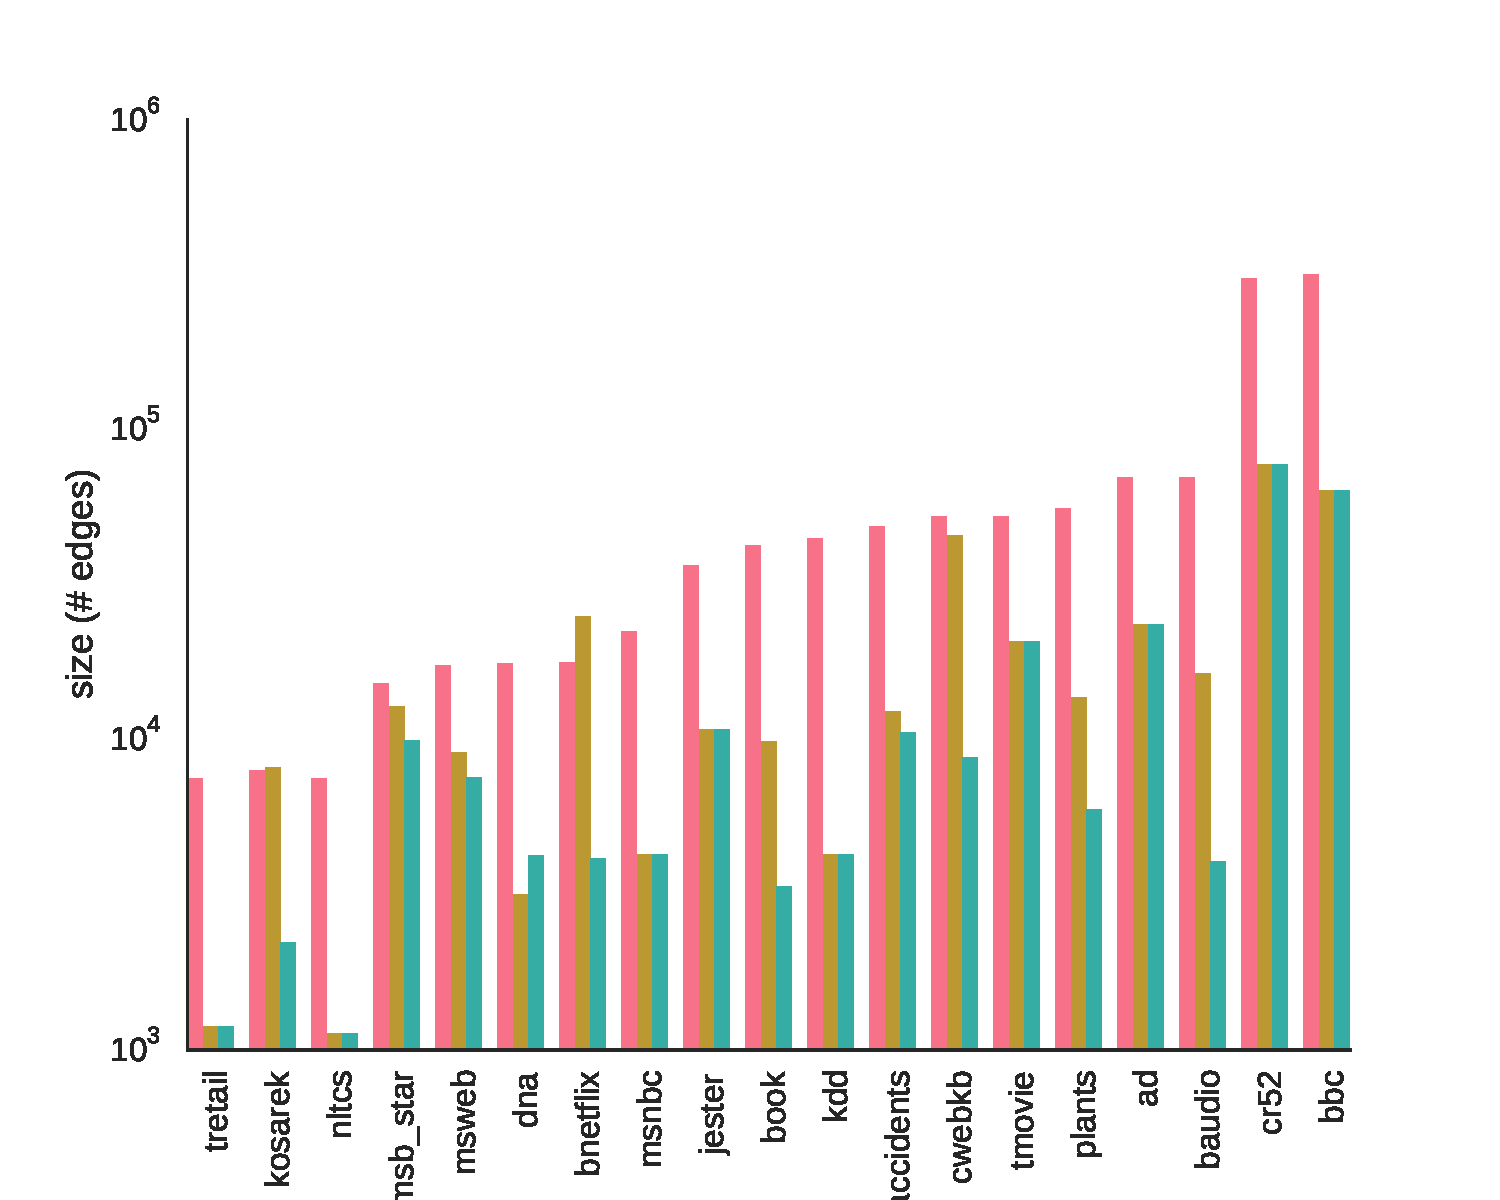
\includegraphics[width=0.4\linewidth]{figures/edges-comp.pdf}&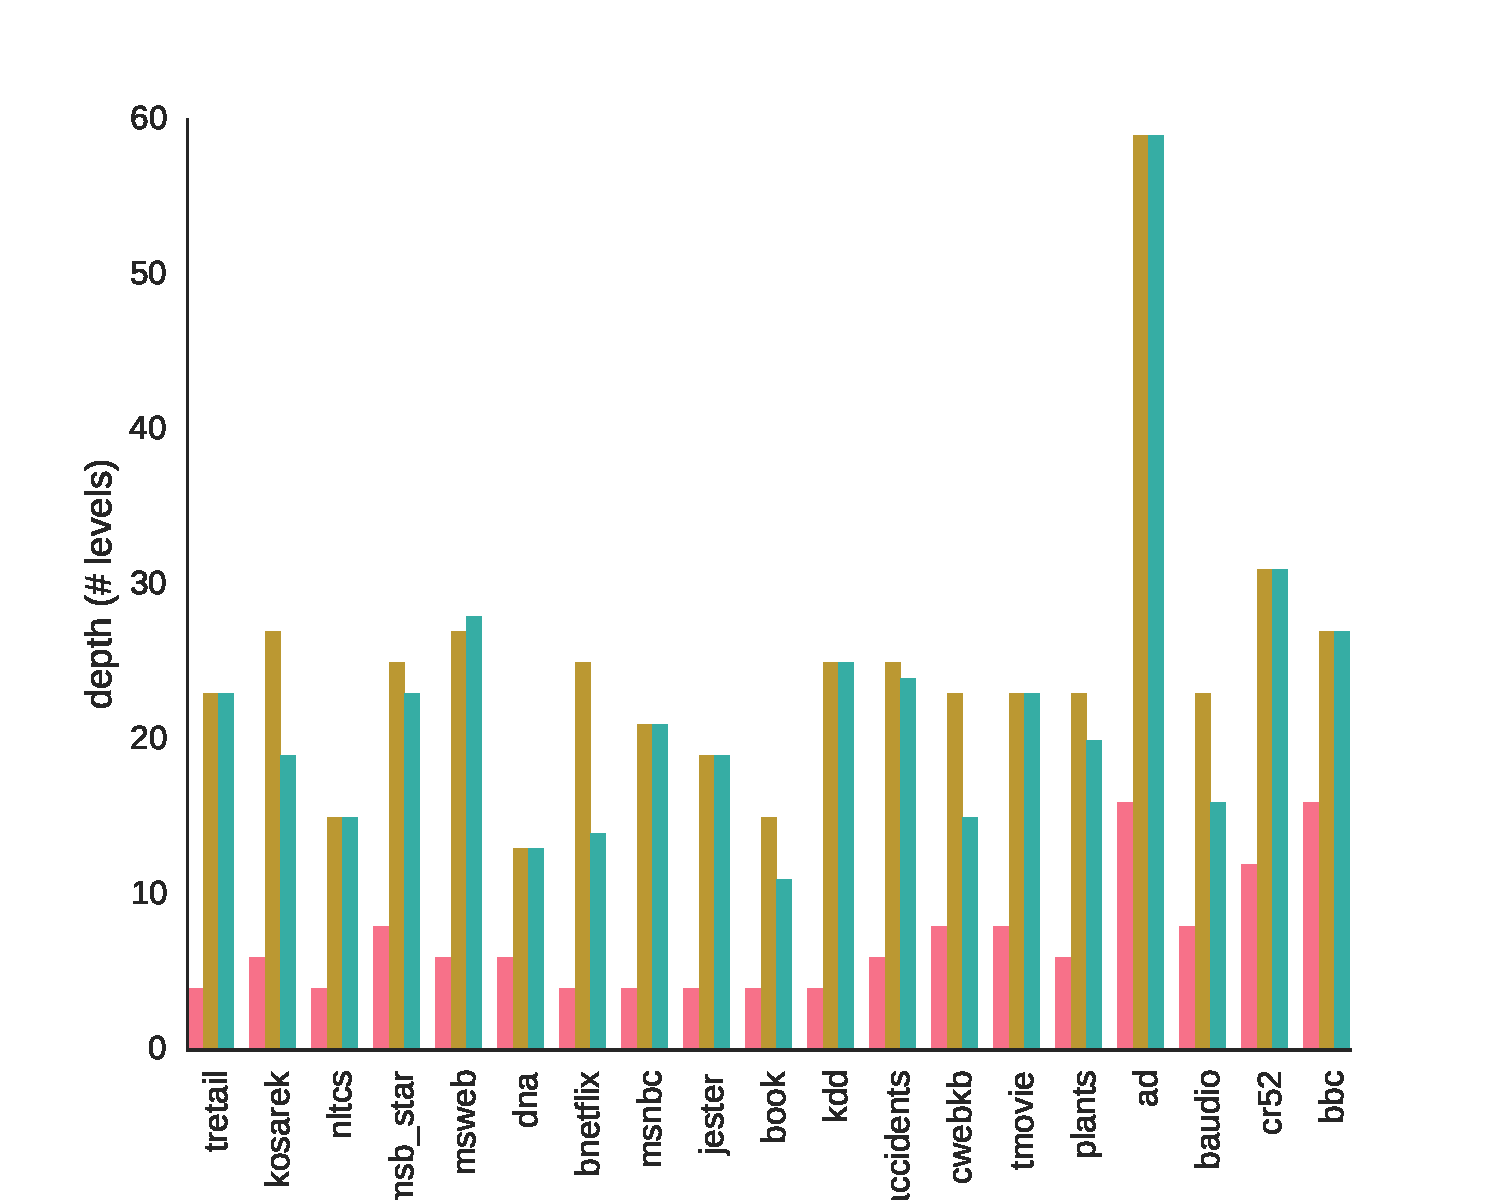
\includegraphics[width=0.4\linewidth]{figures/levels-comp.pdf}
      \end{tabular}
    \end{table}
    \vspace{-20pt}
    \begin{center}
      \begin{minipage}[t]{0.9\linewidth}
        \tiny\flushleft
        Figure 4. Comparing network sizes (left) and depths (right)
        for the networks scoring the best log-likelihoods in the grid
        search as obtained by \textsf{LearnSPN}, \textsf{SPN-B} and
        \textsf{SPN-BT} for each dataset.
      \end{minipage}
    \end{center}\par\bigskip

    \vspace{15pt}
    For \textsf{SPN-BB} and \textsf{SPN-BTB} we simply use the best
    parameters found for \textsf{SPN-B} and \textsf{SPN-BT} using up
    to 50 bootstrapped components; while for
    \textsf{ID-SPN} and \textsf{MT} we reproduce the experiments as
    in~\parencite{Rooshenas2014-short}.\par\bigskip

    Considering the test log-likelihoods, \textsf{SPN-B} improves
    \textsf{LearnSPN} values 6 times, and is surpassed by \textsf{SPN-BT} on 13
    datasets; while \textsf{SPN-BB} and
    \textsf{SPN-BTB} score 11 and 13 wins against \textsf{ID-SPN} respectively.\par\bigskip
    




      \begin{table}[!htbp]
        \centering
        \scriptsize
        \setlength{\tabcolsep}{3pt}  
        \begin{tabular}{r r r r r r r r}
          \toprule
          & \textsf{LearnSPN} & \textsf{SPN-B} & \textsf{SPN-BT} & \textsf{ID-SPN}  & \textsf{SPN-BB}   & \textsf{SPN-BTB}  & \textsf{MT}      \\
          \midrule                                                                                     
          \textbf{NLTCS}      & -6.110            & -6.048         & -6.048          & \textbf{-5.998}  & -6.014            & -6.014            & -6.008           \\
          \textbf{MSNBC}      & -6.099            & -6.040         & -6.039          & -6.040           & \textbf{-6.032}   & -6.033            & -6.076           \\
          \textbf{KDDCup2k}   & -2.185            & -2.141         & -2.141          & -2.134           & -2.122            & \textbf{-2.121}   & -2.135           \\
          \textbf{Plants}     & -12.878           & -12.813        & -12.683         & -12.537          & -12.167           & \textbf{-12.089}  & -12.926          \\
          \textbf{Audio}      & -40.360           & -40.571        & -40.484         & -39.794          & -39.685           & \textbf{-39.616}  & -40.142          \\
          \textbf{Jester}     & -53.300           & -53.537        & -53.546         & \textbf{-52.858} & \textbf{-52.873}  & -53.600           & -53.057          \\
          \textbf{Netflix}    & -57.191           & -57.730        & -57.450         & \textbf{-56.355} & -56.610           & \textbf{-56.371}  & -56.706          \\
          \textbf{Accidents}  & -30.490           & -29.342        & -29.265         & \textbf{-26.982} & -28.510           & -28.351           & -29.692          \\
          \textbf{Retail}     & -11.029           & -10.944        & 10.942          & \textbf{-10.846} & -10.858           & -10.858           & \textbf{-10.836} \\
          \textbf{Pumsb-star} & -24.743           & -23.315        & -23.077         & \textbf{-22.405} & -22.866           & -22.664           & -23.702          \\
          \textbf{DNA}        & -80.982           & -81.913        & -81.840         & -81.211          & -80.730           & \textbf{-80.068}  & -85.568          \\
          \textbf{Kosarek}    & -10.894           & -10.719        & -10.685         & -10.599          & -10.690           & \textbf{-10.578}  & -10.615          \\
          \textbf{MSWeb}      & -10.108           & -9.833         & -9.838          & -9.726           & -9.630            & \textbf{-9.614}   & -9.819           \\
          \textbf{Book}       & -34.969           & -34.306        & -34.280         & -34.136          & -34.366           & \textbf{-33.818}  & -34.694          \\
          \textbf{EachMovie}  & -52.615           & -51.368        & -51.388         & -51.512          & \textbf{-50.263}  & \textbf{-50.414}  & -54.513          \\
          \textbf{WebKB}      & -158.164          & -154.283       & -153.911        & -151.838         & -151.341          & \textbf{-149.851} & -157.001         \\
          \textbf{Reuters-52} & -85.414           & -83.349        & -83.361         & -83.346          & \textbf{-81.544}  & -81.587           & -86.531          \\
          % \textbf{20 NewsG}  & -155.218          & -152.846       & -153.072        & -151.467         &                   &                   & -154.367         \\
          \textbf{BBC}        & -249.466          & -247.301       & -247.254        & -248.929         & \textbf{-226.359} & \textbf{-226.560} & -259.962         \\
          \textbf{Ad}         & -19.760           & -16.234        & -15.885         & -19.053          & -13.785           & \textbf{-13.595}  & -16.012          \\
          \bottomrule
        \end{tabular}
        % \caption[Experimentation results]{\scriptsize Average test
        %   log likelihoods for all algorithms. In bold the best values
        %   after a Wilcoxon signed rank test with $p$-value of 0.05.}
        % \label{tab:resexp}
      \end{table}
      % \vspace{-20pt}
      \begin{center}
        \begin{minipage}[t]{0.9\linewidth}
          \tiny\flushleft
          Table 1. Average test
          log likelihoods for the best networks learned by all
          algorithms on all datasets after the grid search. In bold
          the values that are statistically better than all the others
          according to a Wilcoxon signed rank test with $p$-value of 0.05.
        \end{minipage}
      \end{center}



      
      \end{textblock}


        
  % 
  % section 4
  \begin{textblock}{80}(0, 66.6)
    \usebeamerfont{section name}
    Regularizing by introducing tree distributions as leaves
  \end{textblock}
  
  \begin{textblock}{25.2}(0, 69.1)
    \footnotesize
    LearnSPN regularization is is governed by the hyperparameters $\alpha$ and $m$,
    however using naive factorizations can be ineffective. In order to
    get accurate networks, the algorithm prefers smaller values for
    $m$, resulting in more complex networks\par\bigskip

    Idea: substitute naive factorizations with Bayesian trees as
    \emph{\textbf{multivariate tractable tree
        distributions}}. \textsf{SPN-BT} learns such \textsf{T}rees
    with the Chow-Liu algorithm while stopping the search.\par\bigskip

    \begin{minipage}[t]{0.6\linewidth}
        \flushleft
        Objectives: represent more information allowing for larger
        values of $m$ to be chosen, while preserving tractability for marginals,
        conditionals and MPE inference\\(still linear in the number of leaves).
      \end{minipage}% \hspace{40pt}\begin{minipage}[c]{0.3\linewidth}
    %   \hspace{-30pt}
    %    %\begin{center}
    %     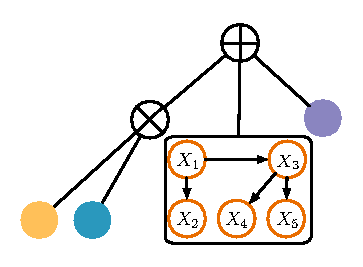
\includegraphics[width=8.2cm]{figures/spn-clt}
    %   %\end{center}
    % \end{minipage}
  \end{textblock}

  \begin{textblock}{10}(15.8, 76.1)
    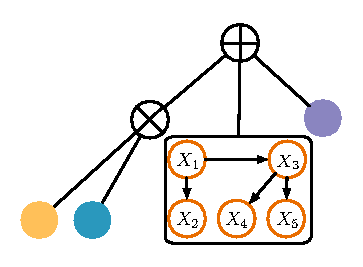
\includegraphics[width=8.2cm]{figures/spn-clt}
    \end{textblock}
  
  \begin{textblock}{25.2}(27.4, 69.1)
    \footnotesize
    \textsf{SPN-BT} reduces the
    size of the networks even more while preserving \textsf{SPN-B}
    accuracy. At larger values of $m$, when both \textsf{SPN-B} and \textsf{LearnSPN}
    accuracies tend to decrease, \textsf{SPN-BT} seems to preserve or
    improve its likelihood.
    
    \begin{center}
      \begin{table}[ht]
        \setlength{\tabcolsep}{30pt}  
        \begin{tabular}{c c}
          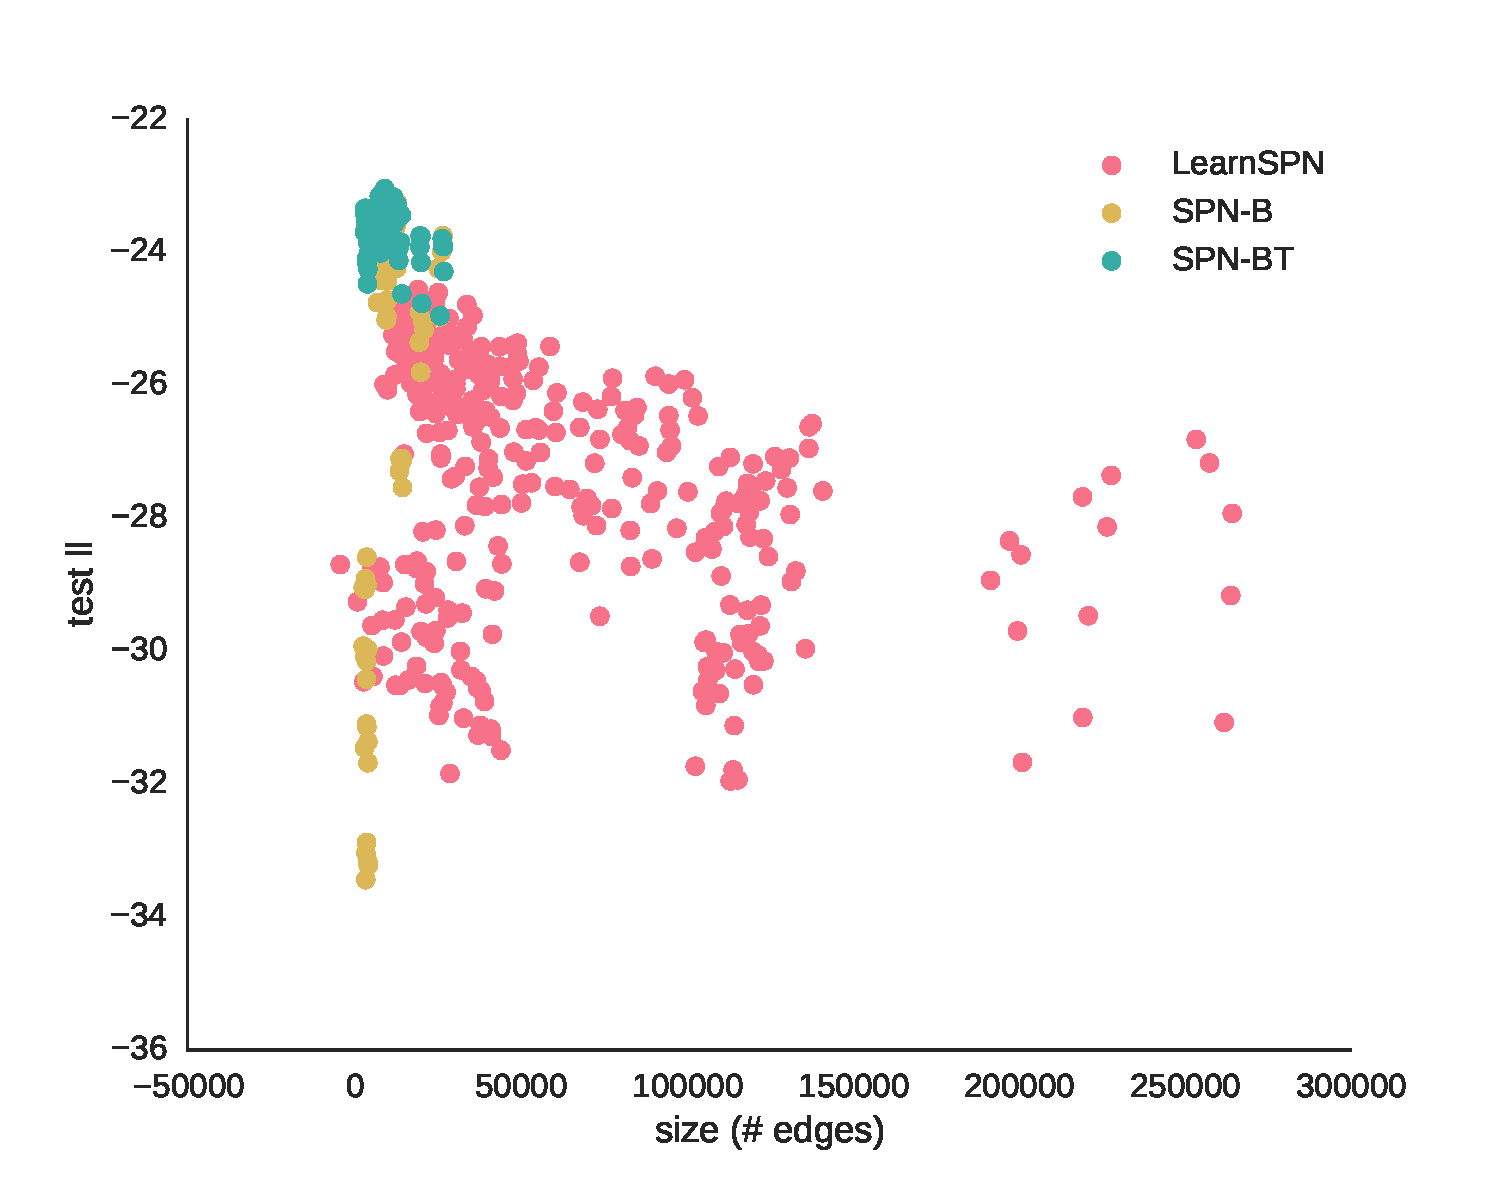
\includegraphics[width=0.4\linewidth]{figures/ll-depth/10-8/pumsb-star-ll-depth}&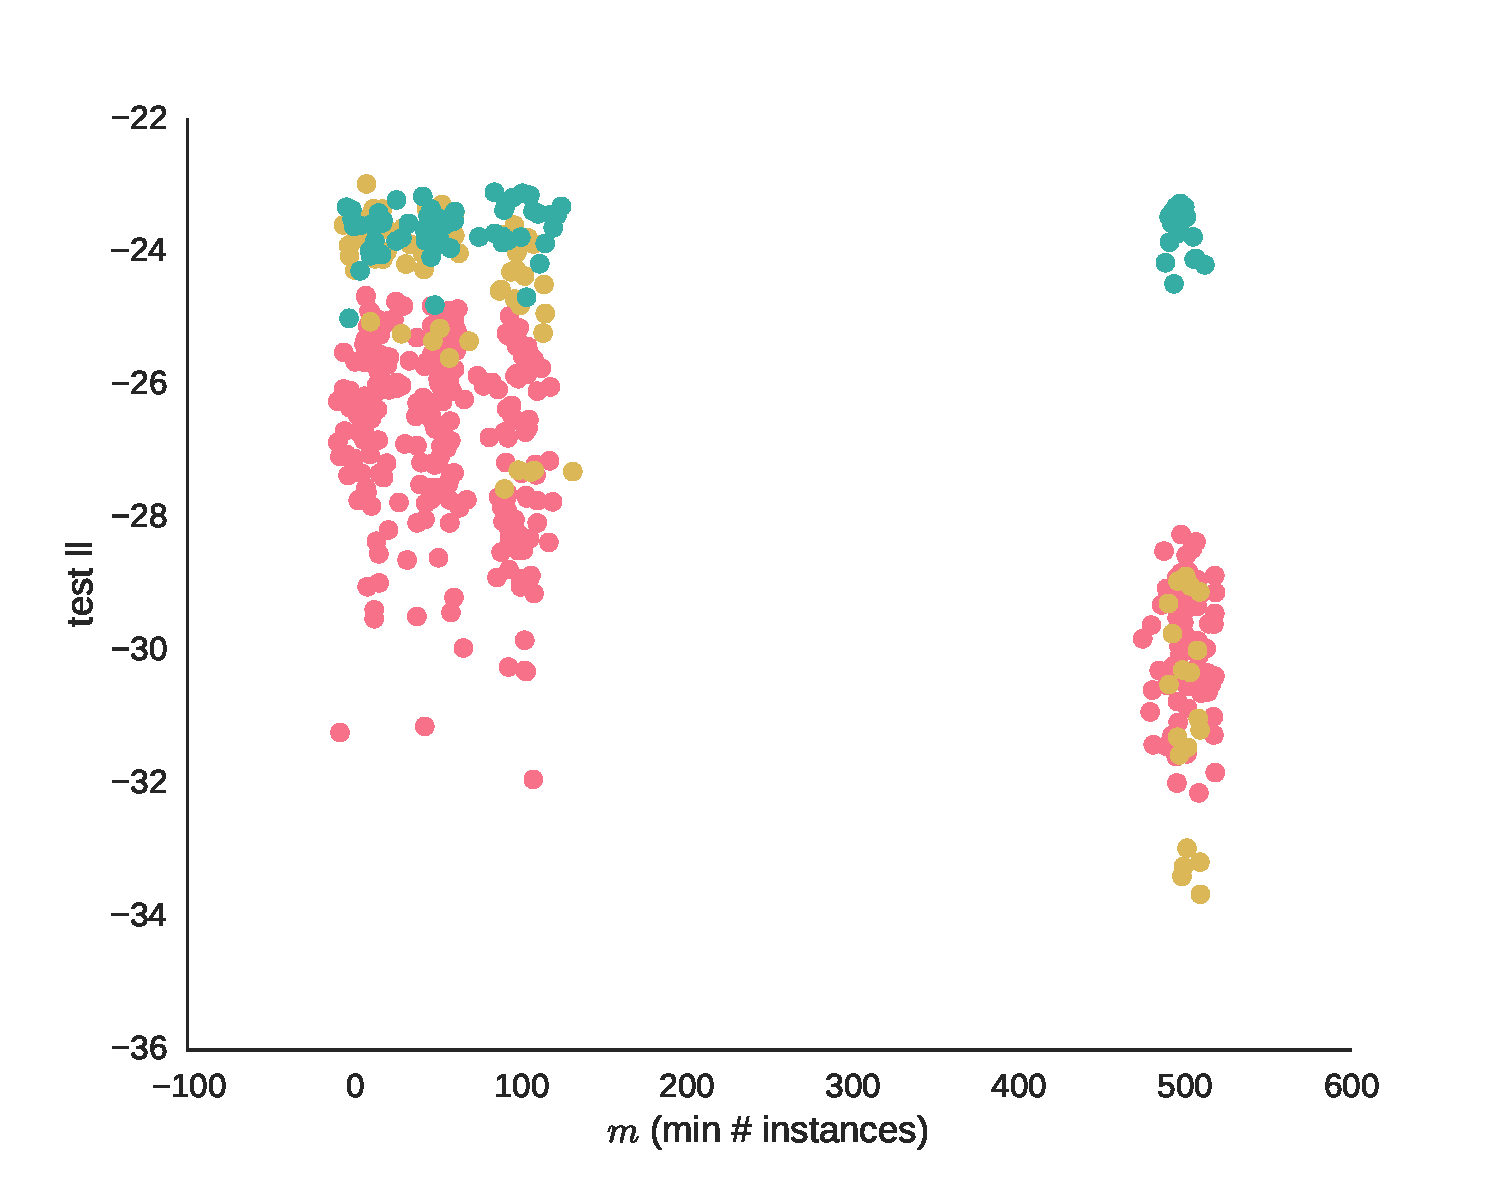
\includegraphics[width=0.4\linewidth]{figures/ll-m/10-8/pumsb-star-ll-m}
        \end{tabular}
      \end{table}
    \end{center}

    \vspace{-20pt}
    \begin{center}
      \begin{minipage}[t]{0.9\linewidth}
        \tiny\flushleft
        Figure 3. Comparing network sizes (left) and values for $m$
        against the  average test
        log-likelihood obtained by \textsf{LearnSPN}, \textsf{SPN-B} and
        \textsf{SPN-BT}
        number of sum node children splits. Each dot is an experiment
        in the grid search performed for the dataset Pumsb-star.
      \end{minipage}
    \end{center}

  \end{textblock}
  
  % \begin{textblock}{25.2}(54.2, 68.4)
  %   \small
  %   \blindtext
  % \end{textblock}
  
  
  % 
  % section 5
  \begin{textblock}{80}(0, 85.3)
    \usebeamerfont{section name}
    Strengthening by model averaging
  \end{textblock}
  
  \begin{textblock}{25.2}(0, 87.8)
    \footnotesize
    The structure building process can still be too greedy and the
    resulting networks not so accurate.\par\bigskip
    
    Idea: interpreting sum nodes as \emph{general additive estimators}
    by leveraging
    classic statistical tools to learn them:
    \textbf{\emph{bagging}}.\par\bigskip

    We draw $k$ bootstrapped samples from the data, then grow an SPN $S_{B_i}$ on
    each of them. Join them into a single SPN $\hat{S}$ with a sum node:
    $\hat{S}=\sum_{i=1}^{k}\frac{1}{k}S_{B_{i}}$.\par\bigskip
    
    Two new variants, \textsf{SPN-BB} and
    \textsf{SPN-BTB}, apply \textsf{B}agging to \textsf{SPN-B} and \textsf{SPN-BT}.\par\bigskip

    Objectives: more robustness and less variance in the model.
    However, the number of nodes can grow exponential if we bootstrap
    $c$ times for each sum node, thus we
    apply it once, at the root level only.

    

  \end{textblock}
  
  \begin{textblock}{25.2}(27.4, 87.8)
    \footnotesize
    Both \textsf{SPN-BB} and \textsf{SPN-BTB} improve their respective
    variants accuracies a lot and beat \textsf{ID-SPN} on 14 datasets
    (see Table 1). Monitoring the test log-likelihood gain can help
    decide the proper number of components.
    \begin{table}[ht]
      \setlength{\tabcolsep}{30pt}  
      \centering
      \begin{tabular}{c c}
        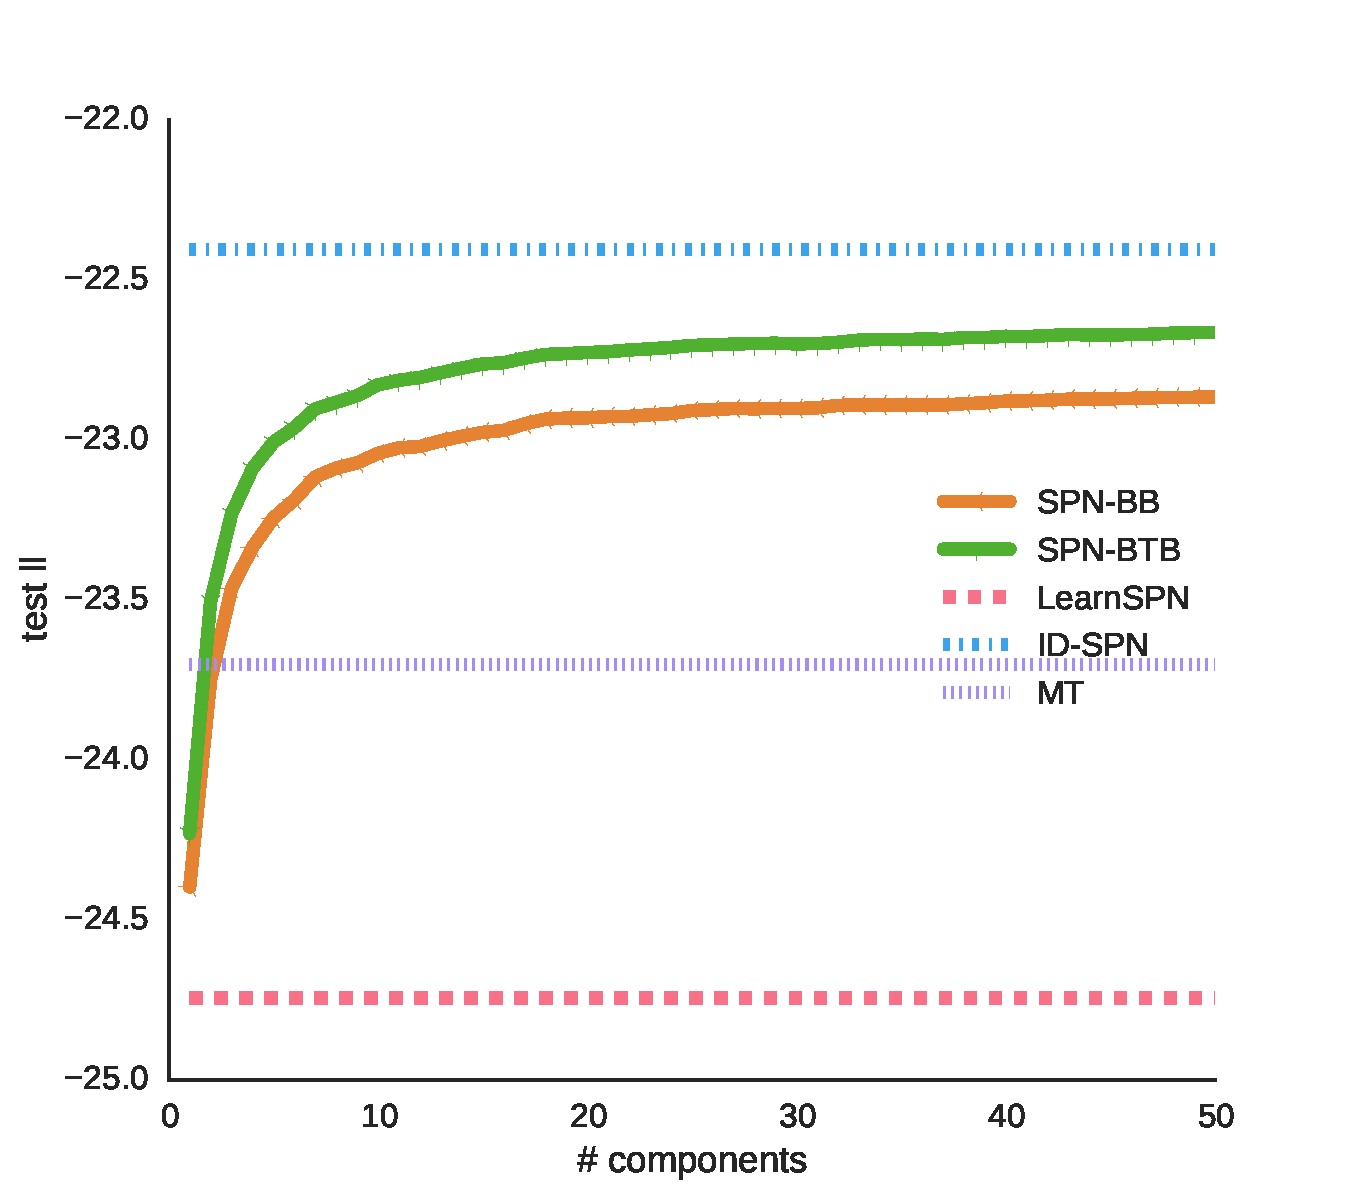
\includegraphics[width=0.4\linewidth]{figures/curves/pumsb-star-png.pdf}&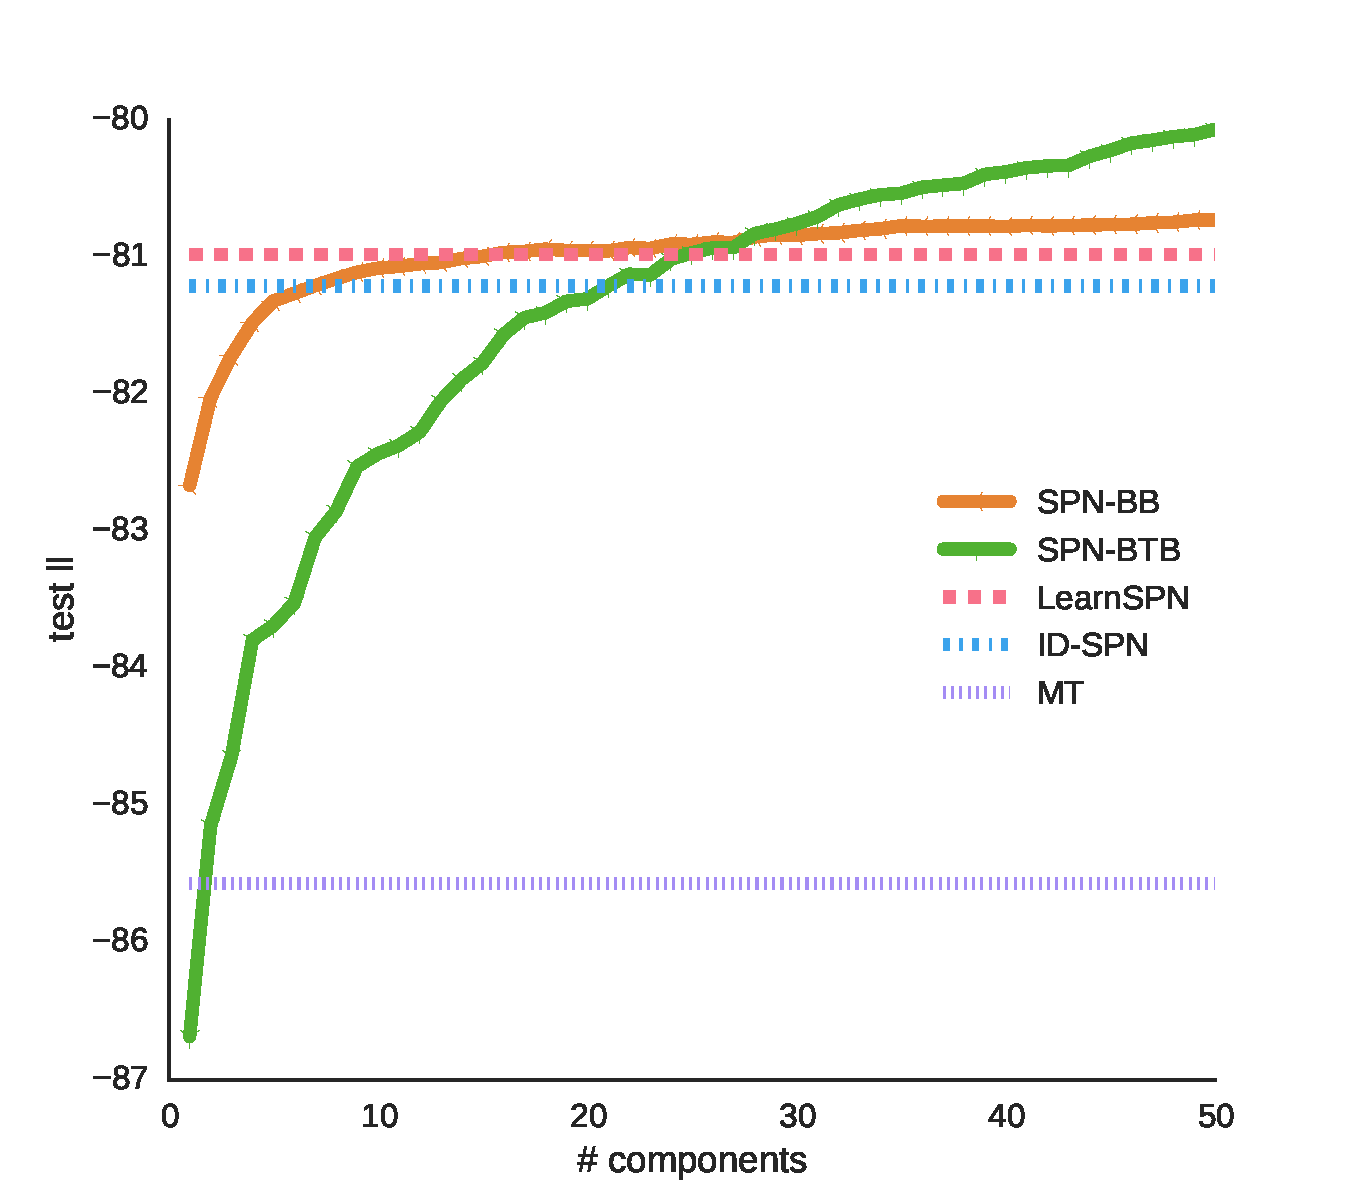
\includegraphics[width=0.4\linewidth]{figures/curves/dna-png.pdf}
      \end{tabular}
    \end{table}
    \vspace{-20pt}
    \begin{center}
      \begin{minipage}[t]{0.9\linewidth}
        \tiny\flushleft
        Figure 3. Comparing test log-likelihoods for \textsf{SPN-BB} and
        \textsf{SPN-BTB} while increasing the number of components against \textsf{LearnSPN}, \textsf{MT} and
        \textsf{ID-SPN} best models accuracies for Pumsb\_star (left)
        and DNA (right).
        .
      \end{minipage}
    \end{center}
  \end{textblock}
  
  % \begin{textblock}{25.2}(54.2, 87.1)
  %   \small
  %   \blindtext
  % \end{textblock}
  
  
  
  % 
  % section 5
  \begin{textblock}{80}(0, 104.)
    \usebeamerfont{section name}
    References
  \end{textblock}
  
  % \begin{textblock}{25.2}(0, 105.8)
  %   \small
  %   % \blindtext
  %   \setlength\bibitemsep{8pt}
  %   \printbibliography
  % \end{textblock}

  \begin{textblock}{52}(0, 106.5)
    \small
    % \blindtext
    \setlength\bibitemsep{8pt}
    \printbibliography
  \end{textblock}
  
  \begin{textblock}{25.2}(27.4, 106.5)
    \small
    % \blindtext
  \end{textblock}
  
  % \begin{textblock}{25.2}(54.2, 105.8)
  %   \small
  %   % \blindtext
  % \end{textblock}

  % 
  % footer
  \begin{textblock}{80}(0, 114.3)
    \usebeamerfont{subtitle}
    \footnotesize
    \textbf{ECML-PKDD 2015} - 8th September 2015, Porto, Portugal\hfill
    {\url{http://www.di.uniba.it/~vergari/code/spyn.html}}
  \end{textblock}
  
\end{frame}




\end{document}

%%% Local Variables:
%%% mode: latex
%%% TeX-master: t
%%% TeX-engine: xetex
%%% End:
